\chapter{Расчет параметров выпрямительной установки возбуждения (ВУВ)}
\section{Определение эксплуатационных характеристик ВУВ}

В качестве ВУВ используем однофазный управляемый двуполупериодный выпрямитель, выполненный по мостовой схеме. При сборе схемы электродинамического торможения, обмотки возбуждения всех тяговых двигателей секции электровоза соединяются последовательно и подключаются к выходу ВУВ. 

Расчетная схема силовой части ВУВ изображена на рисунке~\ref{fig:vuv}.

\begin{figure}[H]
    \centering    
    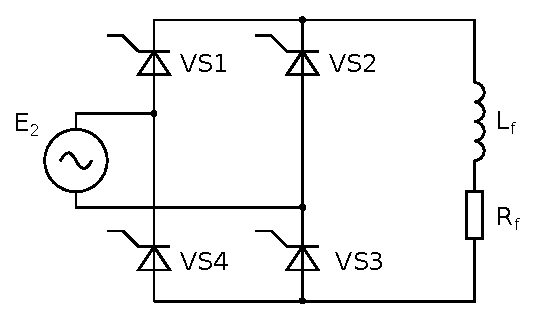
\includegraphics[width=0.5\textheight]{rectifier.eps}
    \caption{Расчетная схема силовой части выпрямительной установки возбуждения: $E_2$ - ЭДС обмотки тягового трансформатора, выделенной для питания ВУВ; VS1~--~VS4 - однооперационные тиристорные ключи; $L_f, \, R_f$ - соответственно, эквивалентная индуктивность и эквивалентное активное сопротивление обмоток возбуждения ТЭД.}
    \label{fig:vuv}
\end{figure}

Нагрузка выпрямительной установки носит активно-индуктивный характер. Ток, протекающий через нагрузку $I_d$ определяется исходя из результата расчетов, приведенных в таблице~\ref{tab:I_field_reg}. Принимаем его $I_d = 857$ А. Максимальное напряжение на зажимах ВУВ расчитываем исходя из эквивалентного сопротивления шести последовательно соединенных обмоток возбуждения

\begin{equation*}
 R_{f} = n_a \, R_{\text{в}} = 6 \cdot 0,03 = 0,18 \, \text{Ом}
\end{equation*}
исходя из чего, по данным таблицы~\ref{tab:I_field_reg}, определяем диапазон регулирования выходного напряжения
\begin{equation*}
 U_d^{\min} = 200 \cdot 0,18 = 36, \, \text{В} \quad U_d^{\max} = 857 \cdot 0,18 = 155, \, \text{В}
\end{equation*}

При минимальном угле открытия тиристоров $\alpha_0 = 9^\circ$ (обеспечивающем надежное их открытие) и с учетом работы на индуктивную нагрузку, расчитаем максимальное среднее значение напряжение на выходе ВУВ
\begin{equation*}
 U_0 = \frac{U_d^{\max}}{\cos \, \alpha_0} = \frac{155}{\cos \, 9^{\circ}} = 157, \, \text{В}
\end{equation*}
Определяем максимальное обратное напряжение на тиристоре, для схемы мостового выпрямителя
\begin{equation*}
 U_{VS}^{\max} = 3,14 \, U_0 = 3,14 \cdot 157 = 493, \, \text{В}
\end{equation*}
Расчетное значение повторяющегося напряжения на тиристоре
\begin{equation*}
 U_{\text{пр}} = k_{U} \, k_{\text{с}} \, U_{VS}^{\max} 
\end{equation*}
где $k_{U} = 1,3 \div 1,5$ - коэффициент запаса по напряжению; $k_{\text{с}} = 1,16$ - коэффициент, учитывающий возможное повышение напряжения в контактной сети до предельного значения 29 кВ, то есть, в нашем случае
\begin{equation*}
 U_{\text{пр}} = 1,4 \cdot 1,16 \cdot 493 = 800, \, \text{В} 
\end{equation*}

Расчетное значение предельного тока тиристора определяем по формуле
\begin{equation*}
 I_{\text{пр}} = k_I \, k_{\text{ф}} \, k_{\text{охл}} \, I_d
\end{equation*}
где $k_I = 1,25 \div 1,4$ - коэффициент запаса по току; $k_{\text{ф}} = 0,9$ - коэффициент формы тока, учитывающий его несинусоидальность; $k_{\text{охл}}$ - коэффициент, учитывающий условия охлаждения тиристоров ($k_{\text{охл}}$ = 2,5 - при стандартном радиаторе без обдува; $k_{\text{охл}} = 1,0$ - при принудительном воздушном охлаждении. Тогда, в нашем случае

\begin{equation*}
 I_{\text{пр}} = 1,25 \cdot 0,9 \cdot 1,0 \cdot 857 = 964 \approx 1000, \, \text{А}
\end{equation*}

Тиристор выбираем из условия 
\begin{equation*}
 U_{\text{п}} \ge U_{\text{пр}}, \quad I_{\text{п}} \ge I_{\text{пр}}
\end{equation*}
где $U_{\text{п}}$ - максимально допустимое мгновенное напряжение, прикладываемое к тиристору; $I_{\text{п}}$ - предельное значение тока тиристора.

Указанным условиям удовлетворяет тиристор  марки T133-500 производства ПАО <<Электровыпрямитель>> (г.~Саранск).

Тиристор Т133-500 имеет исполнение таблеточного типа в корпусе PT31. Технические характеристики тиристора указаны в нижеприведенной таблице

\begin{figure}[H]
    \centering        
    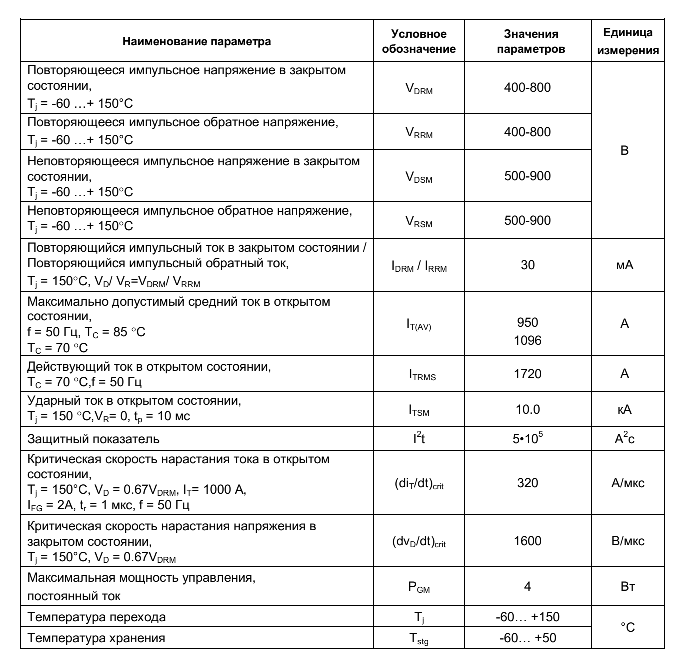
\includegraphics[width=0.6\textheight]{T133-500.eps}    
    \label{fig:T133-500}
\end{figure}





